% !TEX encoding = UTF-8 Unicode
\documentclass[10pt,twoside]{book}\usepackage[T1]{fontenc}
\usepackage{tikz}

\usepackage[active,tightpage,xetex]{preview}

\usepackage{fontspec,xunicode}

\PreviewEnvironment{pgfpicture}

\setlength\PreviewBorder{0pt}

\usetikzlibrary{calc}

\usetikzlibrary{positioning}



\usepackage{fontspec,xunicode}

\setmainfont{Open Sans Condensed Light}
\begin{document}
\begin{tikzpicture}
\node[anchor=south west,inner sep=0] (image) at (0,0) {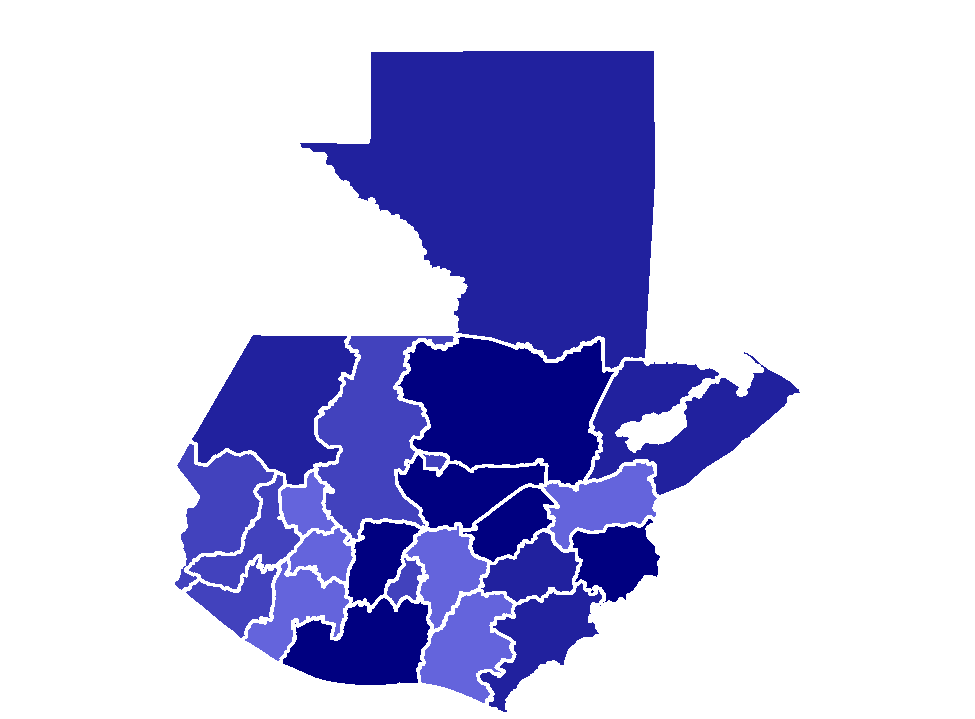
\includegraphics{mapa}};
\begin{scope}[x={(image.south east)},y={(image.north west)}]
\draw[help lines,xstep=.1,ystep=.1] (0,0) grid (1,1);
\foreach \x in {0,1,...,9} { \node [anchor=north] at (\x/10,0) {0.\x}; }
\foreach \y in {0,1,...,9} { \node [anchor=east] at (0,\y/10) {0.\y}; }
% ###############ALTA VERAPAZ############################## %
\draw [thick] (0.5,0.4) -- (0.5,0.9);
\filldraw (0.5,0.4) circle (1pt);
\draw [thick] (0.4989,0.9) -- (0.73,0.9);
\node[text width=3cm] at (0.83,0.9) {Alta Verapaz \\ 5\%};

% ###############BAJA VERAPAZ############################## %
\draw [thick] (0.525,0.33) -- (0.525,0.81);
\filldraw (0.525,0.33) circle (1pt);
\draw [thick] (0.525,0.81) -- (0.73,0.81);
\node[text width=3cm] at (0.83,0.81) {Baja Verapaz \\ 5\%};

%#############EL PROGRESO################################# %
\draw [thick] (0.55,0.28) -- (0.55,0.72);
\filldraw (0.55,0.28) circle (1pt);
\draw [thick] (0.55,0.72) -- (0.73,0.72);
\node[text width=3cm] at (0.83,0.72) {El Progreso \\ 5\%};


% ###############PETEN############################## %
\draw [thick] (0.58,0.55) -- (0.58,0.63);
\filldraw (0.58,0.55) circle (1pt);
\draw [thick] (0.58,0.63) -- (0.73,0.63);
\node[text width=3cm] at (0.83,0.63) {Petén \\ 5\%};

%#############IZABAL################################# %
\draw [thick] (0.64,0.45) -- (0.64,0.55);
\filldraw (0.64,0.45) circle (1pt);
\draw [thick] (0.6389,0.55) -- (0.73,0.55);
\node[text width=3cm] at (0.83,0.55) {Izabal \\ 5\%};



%#############ZACAPA################################# %
\filldraw (0.62,0.31) circle (1pt);
\draw [thick] (0.62,0.33) -- (0.73,0.33);
\draw [thick] (0.62,0.31) -- (0.62,0.33);
\node[text width=3cm] at (0.83,0.33) {Zacapa \\ 45\%};


%#############CHIQUIMULA################################# %
\filldraw (0.63,0.22) circle (1pt);
\draw [thick] (0.63,0.25) -- (0.73,0.25);
\draw [thick] (0.63,0.22) -- (0.63,0.25);
\node[text width=3cm] at (0.83,0.25) {Chiquimula \\ 15\%};

%#############JALAPA################################# %
\filldraw (0.55,0.22) circle (1pt);
\draw [thick] (0.55,0.17) -- (0.73,0.17);
\draw [thick] (0.55,0.22) -- (0.55,0.17);
\node[text width=3cm] at (0.83,0.17) {Jalapa \\ 15\%};

%#############JUTIAPA################################# %
\filldraw (0.57,0.12) circle (1pt);
\draw [thick] (0.57,0.10) -- (0.73,0.10);
\draw [thick] (0.57,0.12) -- (0.57,0.10);
\node[text width=3cm] at (0.83,0.09) {Jutiapa \\ 15\%};

%#############SANTA ROSA################################# %
\filldraw (0.48,0.11) circle (1pt);
\draw [thick] (0.48,0.01) -- (0.73,0.01);
\draw [thick] (0.48,0.11) -- (0.48,0.01);
\node[text width=3cm] at (0.83,0.01) {Santa Rosa \\ 15\%};

% ###############QUICHE############################## %
\draw [thick] (0.39,0.35) -- (0.39,0.9);
\filldraw (0.39,0.35) circle (1pt);
\draw [thick] (0.39,0.9) -- (0.20,0.9);
\node[align=right, text width=3cm] at (0.10,0.9) {Quiché \\ 5\%};


% ###############SOLOLÁ############################## %
\draw [thick] (0.34,0.23) -- (0.34,0.81);
\filldraw (0.34,0.23) circle (1pt);
\draw [thick] (0.34,0.81) -- (0.20,0.81);
\node[align=right,text width=3cm] at (0.1,0.81) {Sololá \\ 5\%};

% ###############TOTONICAPAN############################## %
\draw [thick] (0.31,0.29) -- (0.31,0.72);
\filldraw (0.31,0.29) circle (1pt);
\draw [thick] (0.31,0.72) -- (0.20,0.72	);
\node[align=right,text width=3cm] at (0.1,0.72) {Totonicapán \\ 5\%};

% ###############QUETZALTENANGO############################## %
\draw [thick] (0.28,0.26) -- (0.28,0.63);
\filldraw (0.28,0.26) circle (1pt);
\draw [thick] (0.28,0.63) -- (0.20,0.63	);
\node[align=right,text width=3cm] at (0.10,0.63) {Quetzaltenango \\ 5\%};


\end{scope}
\end{tikzpicture}
\end{document}
